\chapter{修士作品 《Grasp(er)》}
\label{about_grasper}
本章では、修士作品《Grasp(er)》の概要と、その制作プロセスを説明する。

\section{作品概要}
\begin{figure}[H]
  \centering
  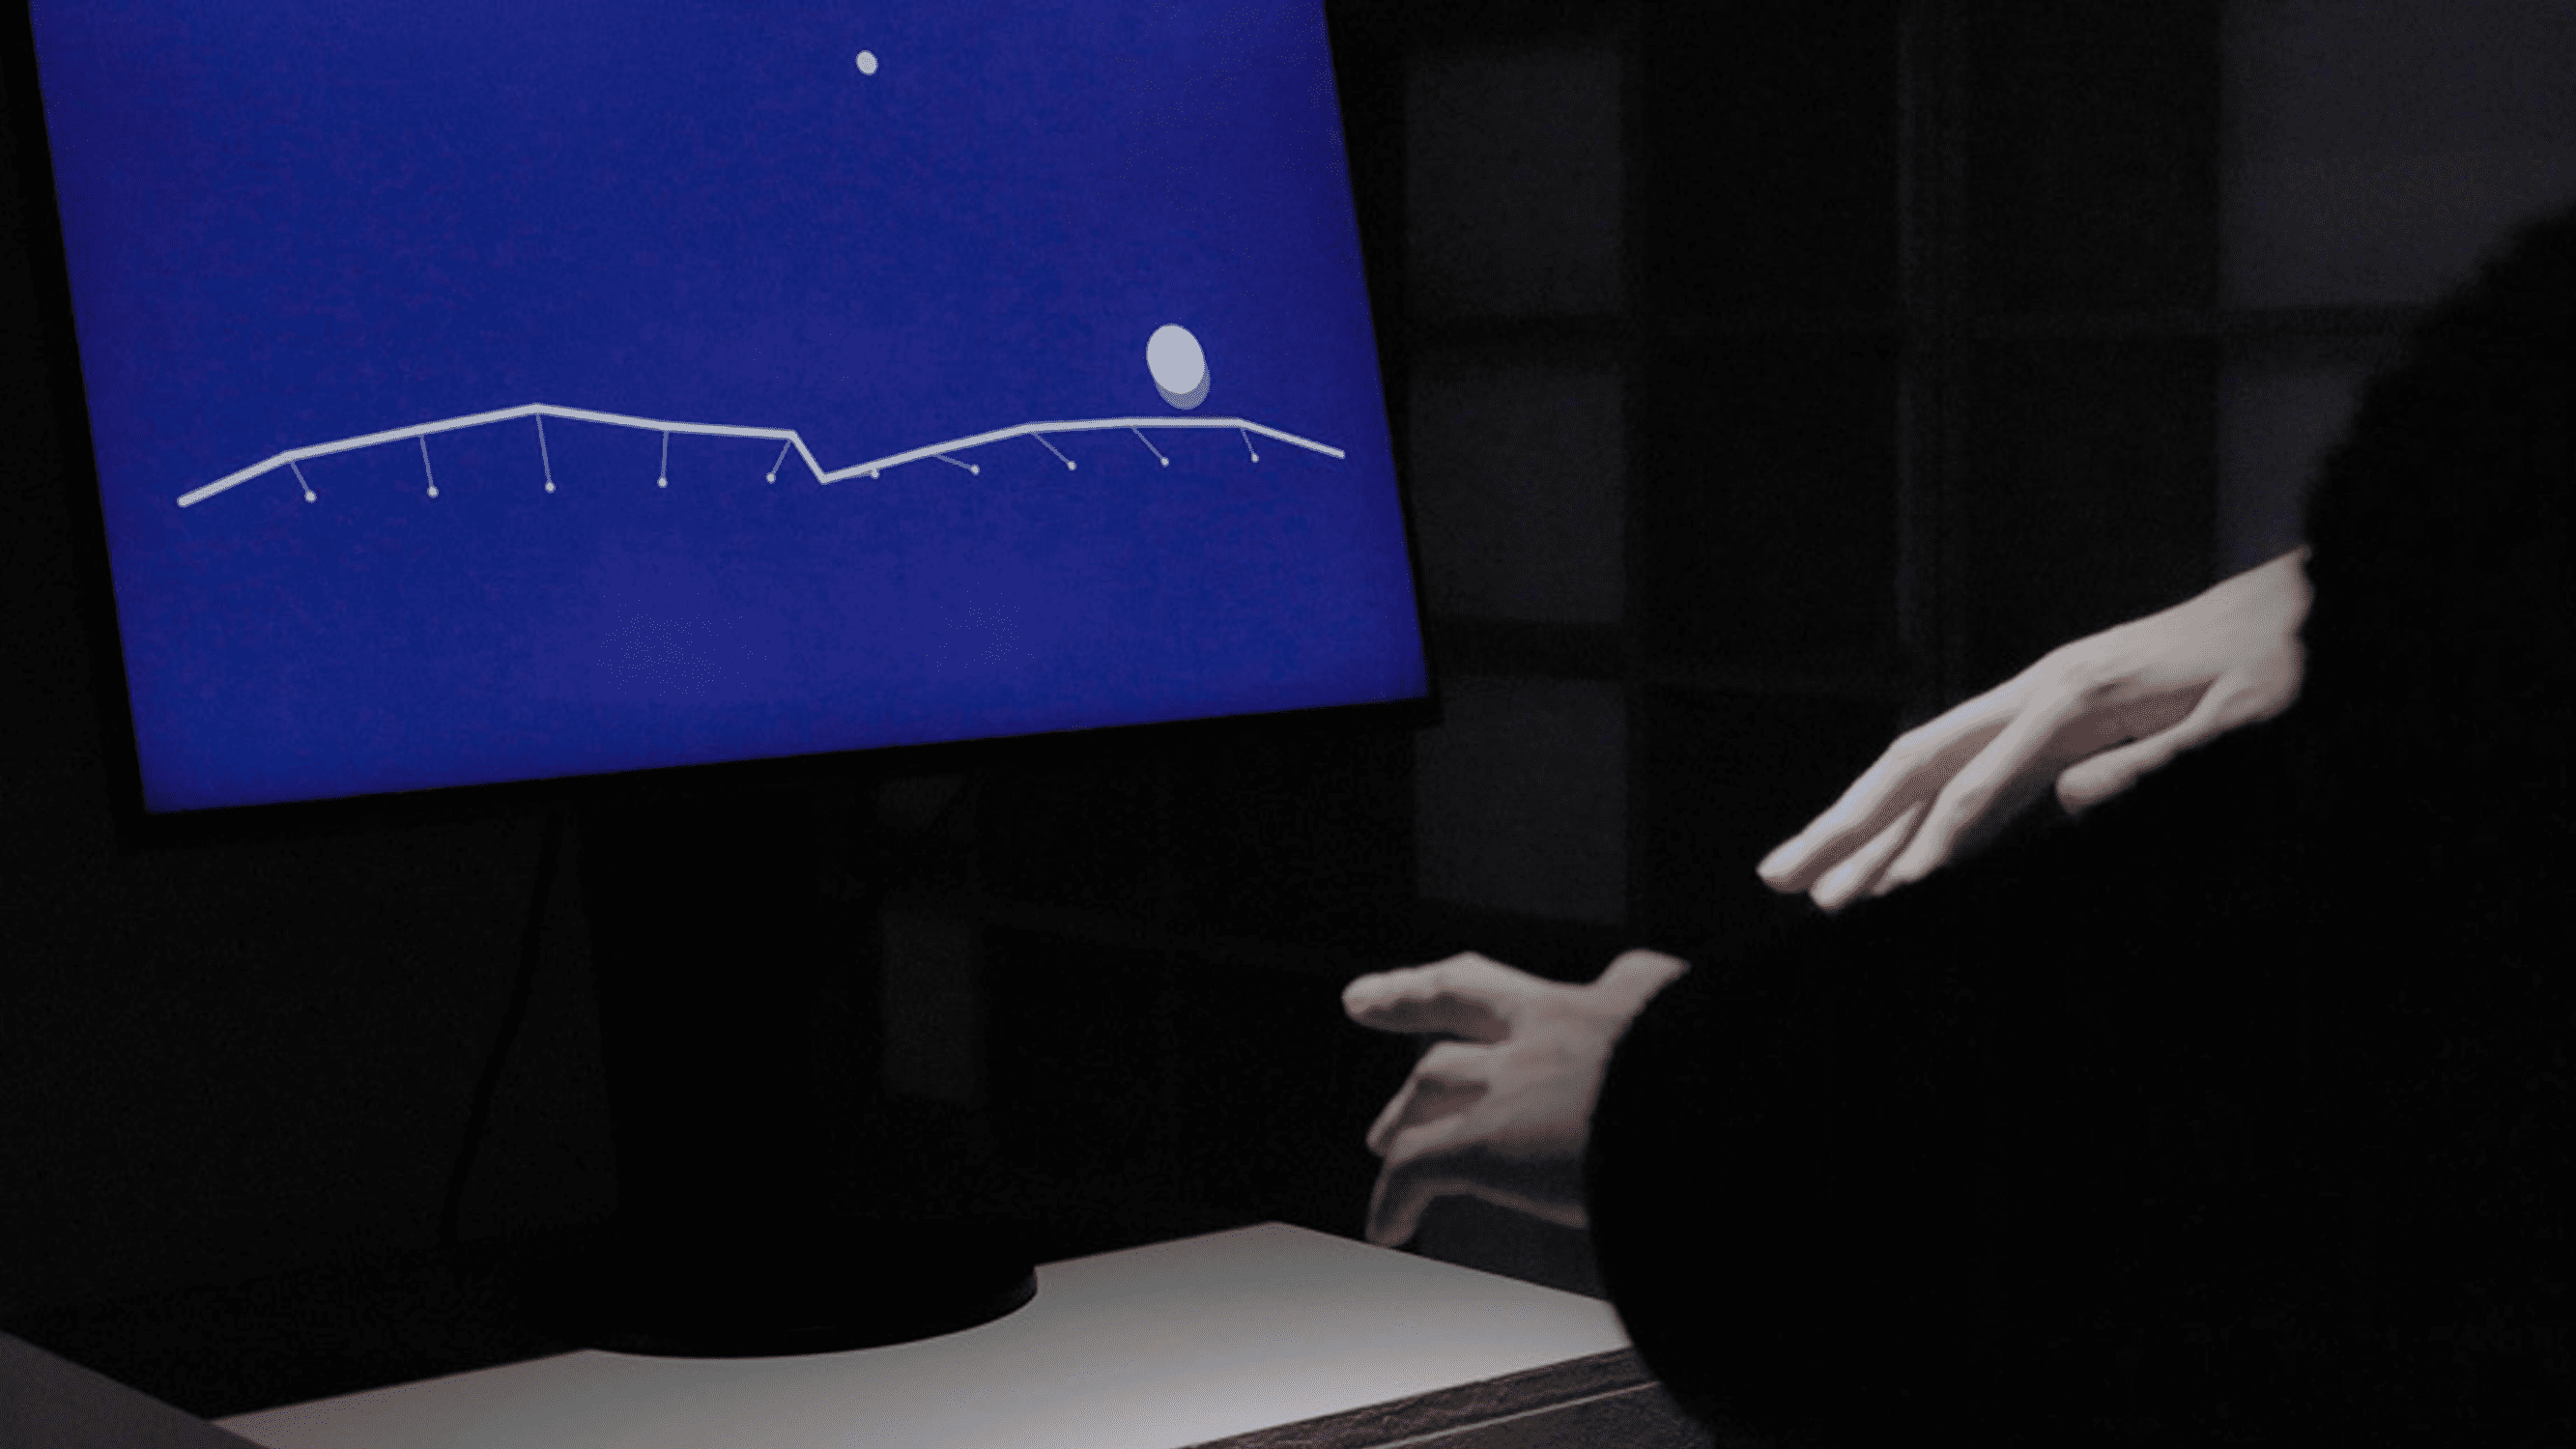
\includegraphics[width=15cm]{img/thumbnail.png}
  \caption{修士作品《Grasp(er)》}
  \label{grasper}
\end{figure}

《Grasp(er)》は、「Familiar / Strange」と「Relation」という二つから構成された作品群である。手の形が大きく変化したり、その変化した手指を使った細かな操作が求められる中で芽生える、身体の他者性に対する注目を扱った作品である。

最初はうまくいかず「もどかしさ」を感じながらも、試行錯誤や意識的な身体動作を行う期間を経て折り合いをつけていく過程に、「変化」が起こる。高度な道具の能力を享受するだけでなく、\textit{grasp}を通して、人が能力を身につけるという側面に着目して、作品名を《Grasp(er)》とした。

以下では、本作を構成する2つの作品について説明する。

% これらに共通するのは、\textit{grasp}の中で個人が目的意識や興味を抱くことで、\textit{grasp}が連鎖的に生じることである。

% 制作者は「このようなことをしてほしい」という行為の中身を設計せず、体験する個人がその中で次々と注目する対象を見出すことによって、個人が行為を創造していくことを目指している。このため、「手指の構造や、手指を取り巻く環境を変化させることで、手指の運動に注目する構造」を作ることに取り組んだ。このときの「注目」が起点となって\textit{grasp}の期間が生じるが、その先々で起こる体験は個人に委ねられ、明示的な目的は設定されていない。

\subsection*{Familiar / Strange}
\begin{figure}[H]
  \centering
  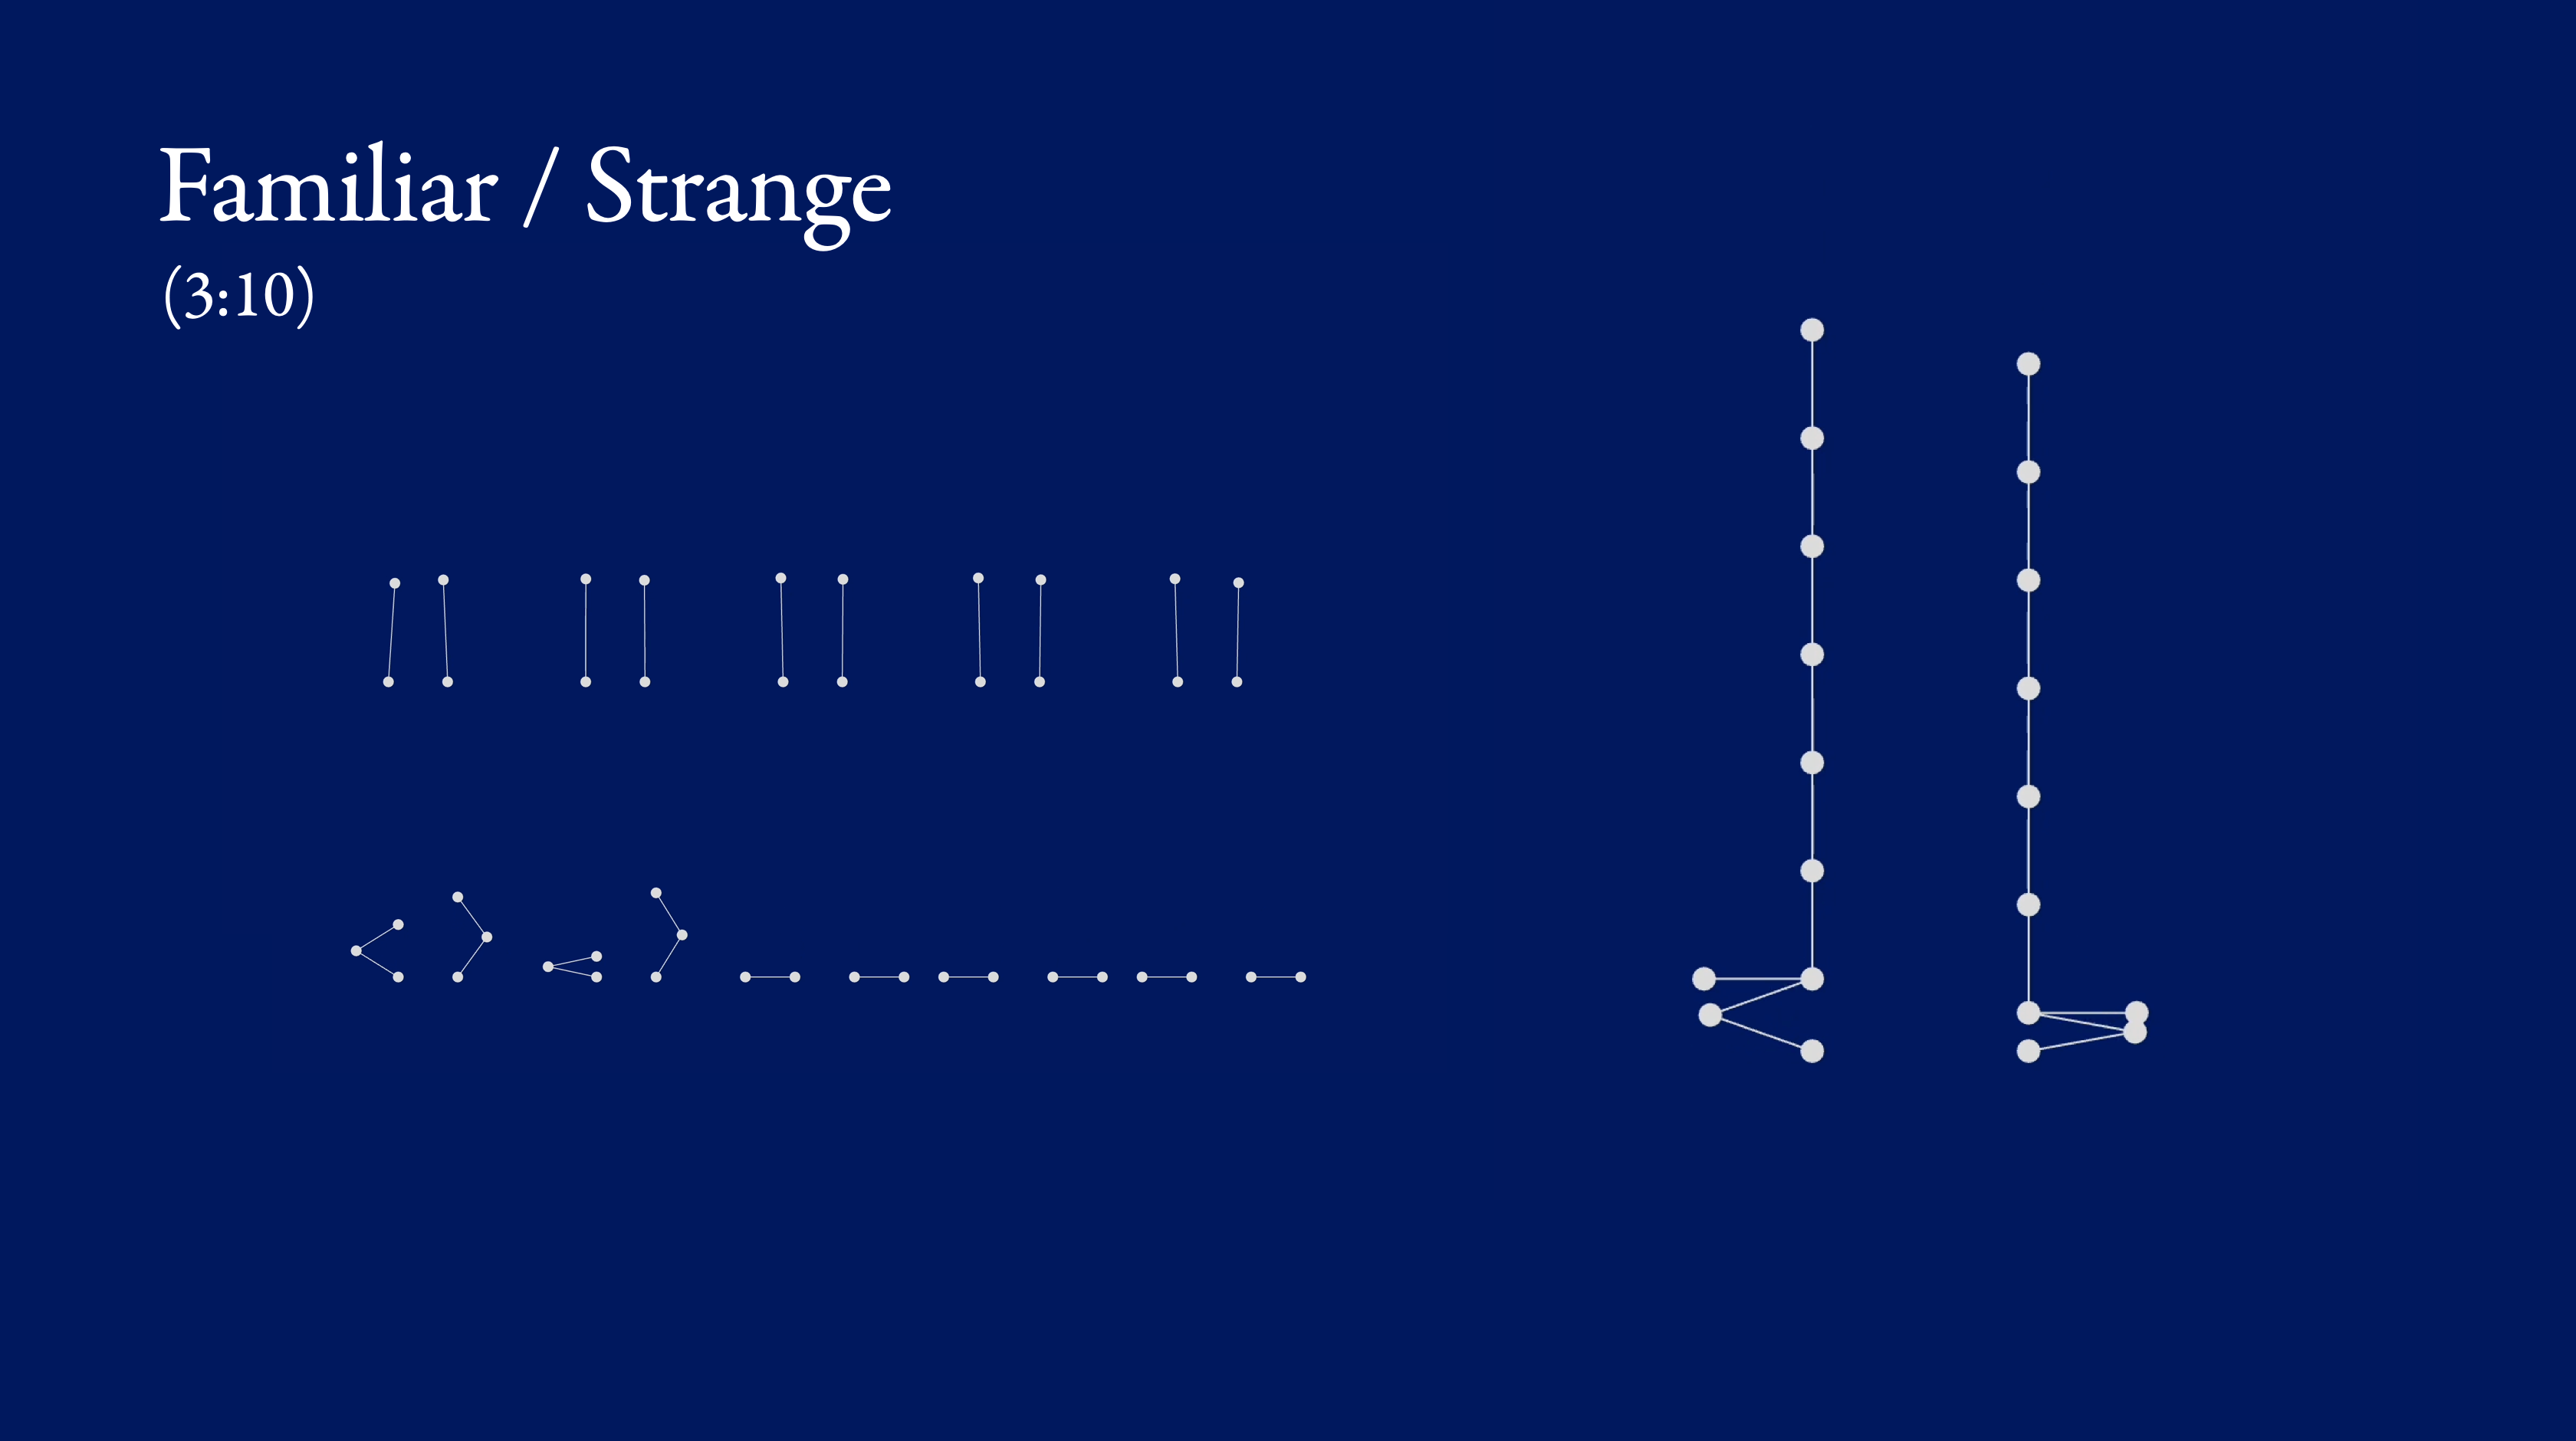
\includegraphics[width=15cm]{img/fs-02.png}
  \caption{Familiar / Strange}
  \label{fig:familiar_strange}
\end{figure}
「Familiar / Strange」は、手指の配置や関節の数・位置が次々と変化していく作品で、手の運動に対する再注目が起きることを目指している。作品は最初、手の形がそのまま現れた状態から開始し、指の並びや関節の配置の変化が起きる。一本一本の指がくの字の形をして積み上げられる様子をピークに、逆順に変化が巻き戻され、再び元の手の形に戻るという、3分10秒で1ループの構造となっている。


変換の過程は、イージングやゴム紐が切れた時のような振動を伴う動きによって補完される。シーン遷移を説明する図を以下に示す。
\begin{figure}[H]
  \centering
  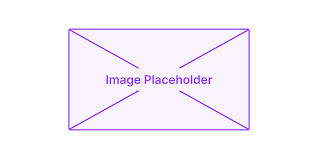
\includegraphics[width=15cm]{img/placeholder.png}
  \caption{Familiar / Strangeにおけるシーン遷移}
  \label{fig:diagram_familiar_strange}
\end{figure}

\subsection*{Relation}
\begin{figure}[H]
  \centering
  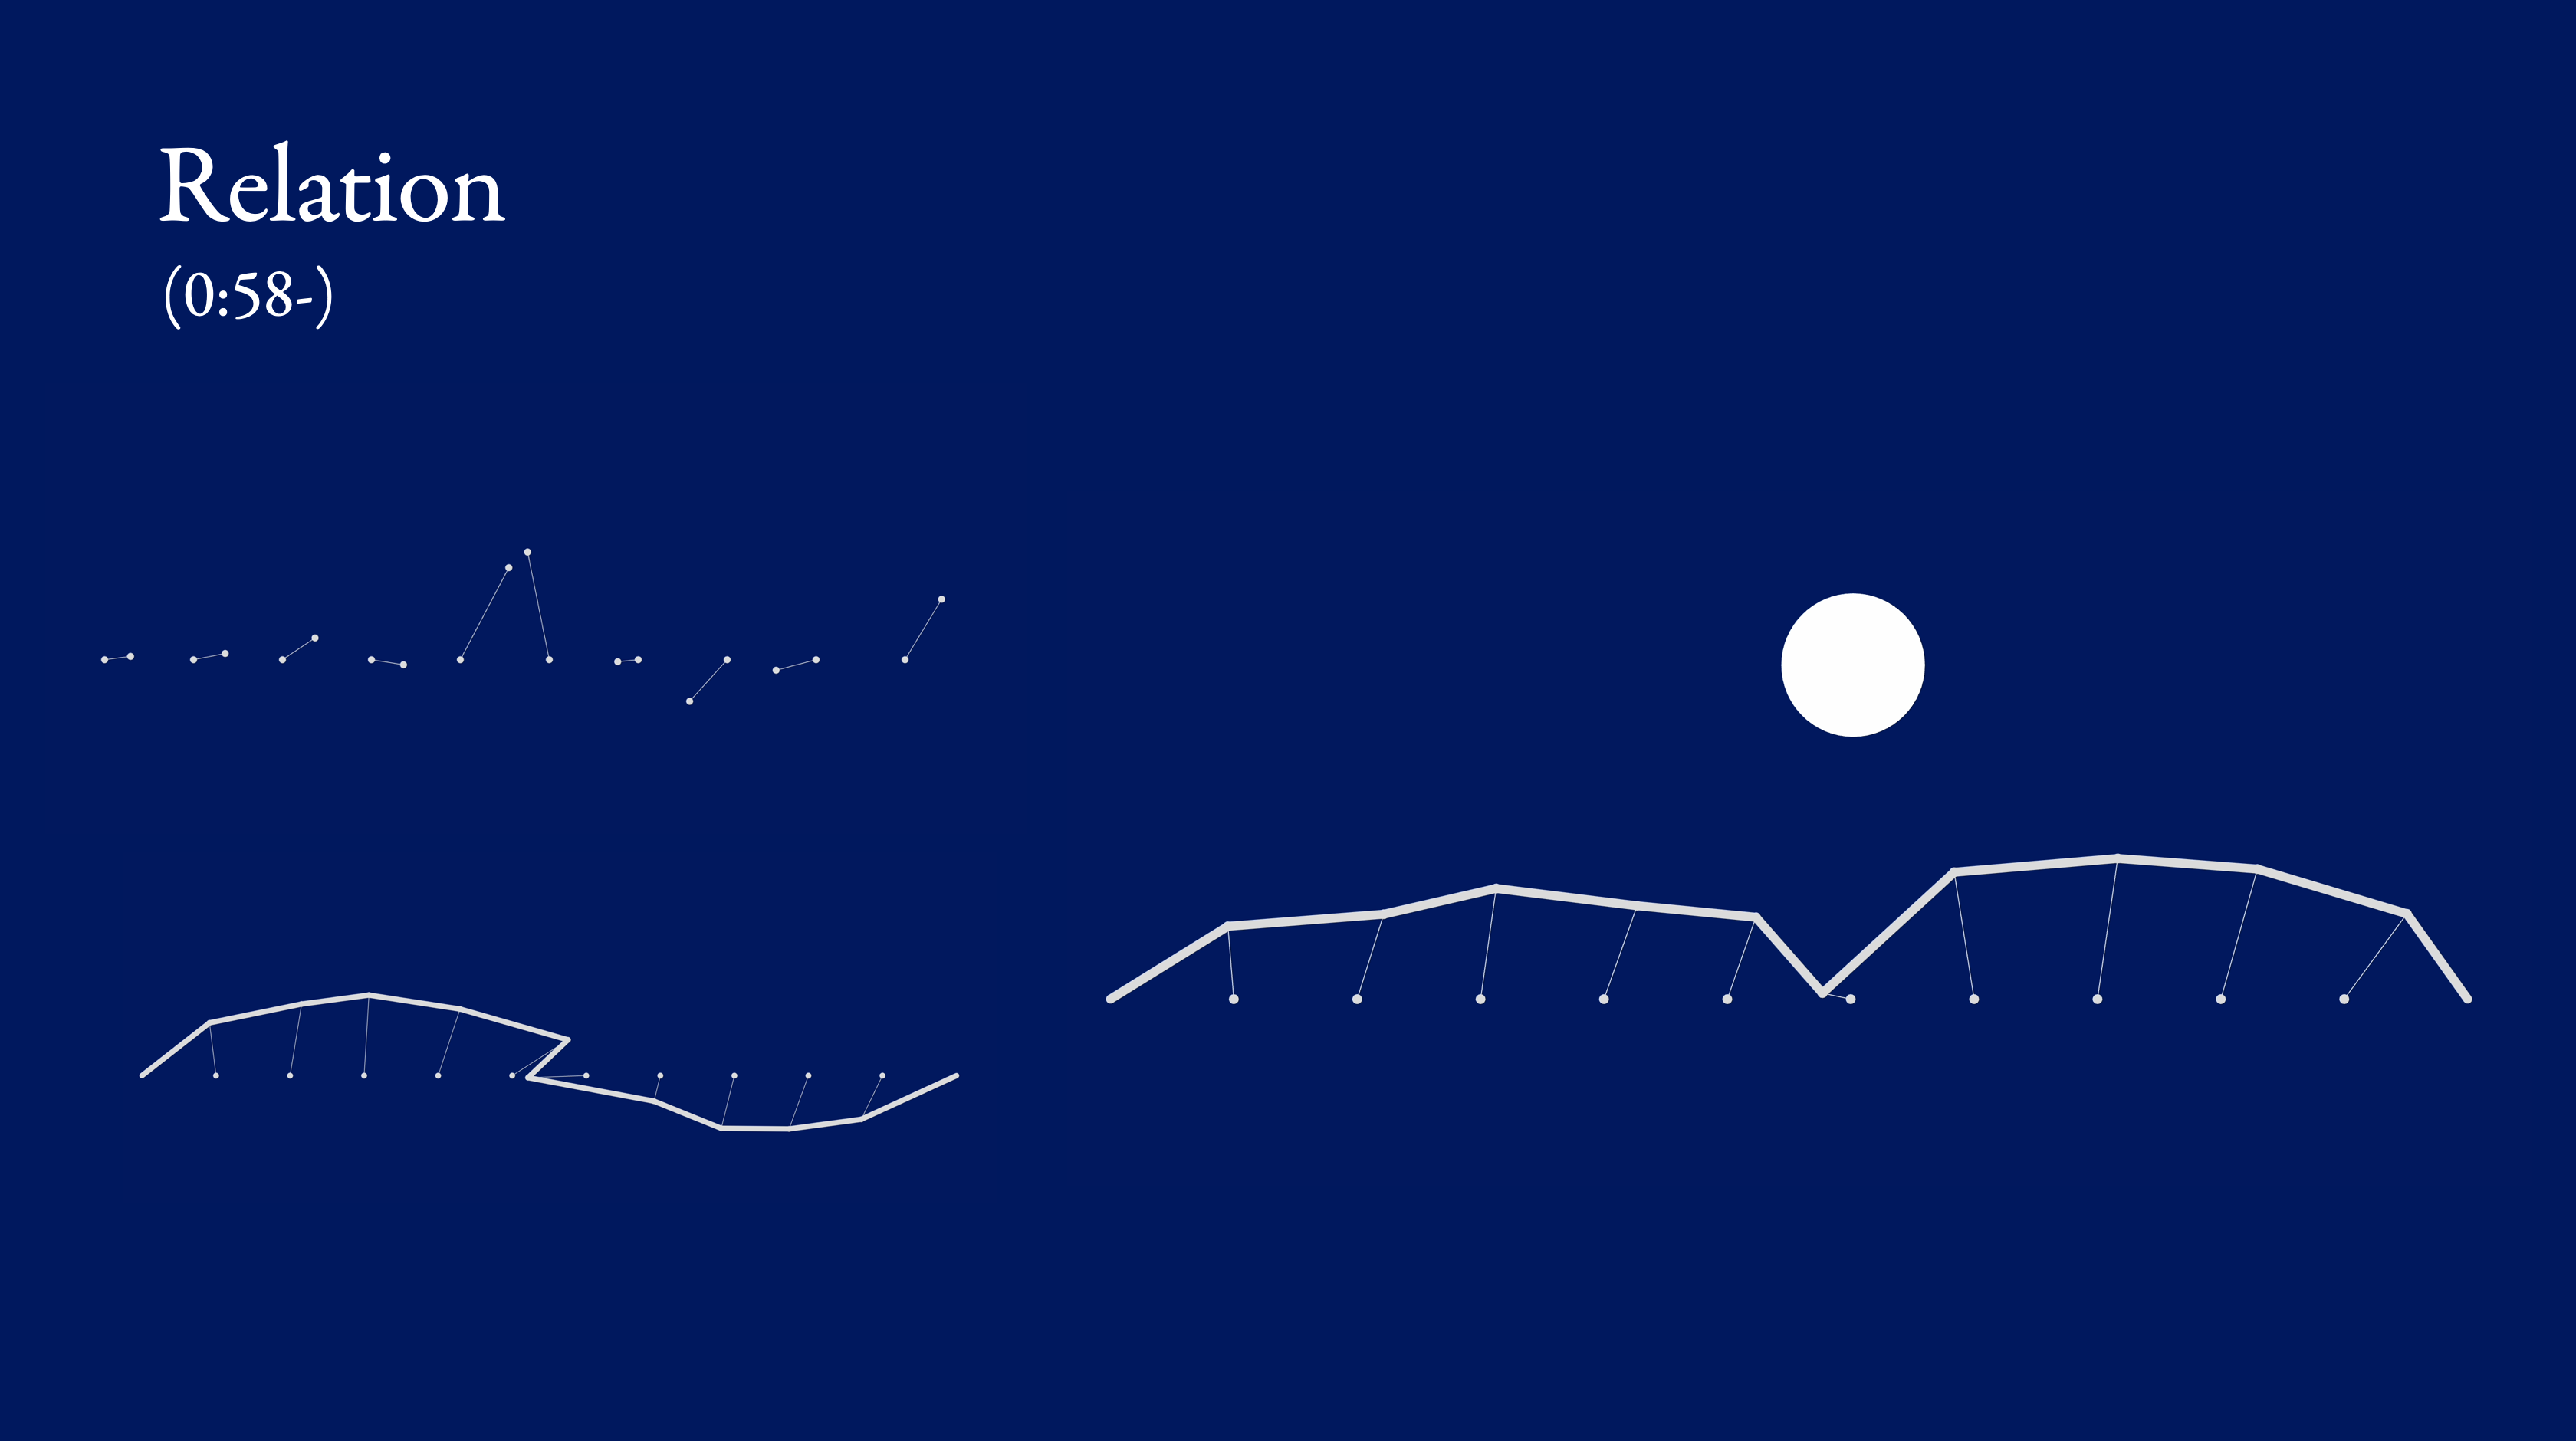
\includegraphics[width=15cm]{img/relation.png}
  \caption{Relation}
  \label{fig:relation}
\end{figure}
「Relation」は、変化した手指を取り巻く関係が次々と変化していく作品で、手と直接的に制御できないボールの関係性におけるGraspに焦点を当てている。1つ目の作品と同様、最初は手が表示された状態から始まり、段階的に並び替えられた手指を覆う皮膜が現れ、ボールが現れる。最後はマトが現れ、的を取るたびにボールの大きさが小さくなり、3つ連続して取ると、皮膜は消え、再び元の手の形に戻る。

トラッキングされた手指の位置が、手首から指ごとに分割され、左端から右へ、左手の小指から親指、そして右手の親指から小指の順に整列される。しばらくすると、指先以外の運動が捨象され、残された指先を結ぶ線が現れる。ここで、現れた線によって再び全ての指が1つのまとまりとして統合されることになるが、その線は後に現れるボールに対して衝突判定が適用される、新しい構造の手指を覆う皮膜のような機能を有する。皮膜のある領域を外れるとボールは落下するが、そのあとは再び画面の中央にボールが出現する。

さらに一定時間が経過すると、皮膜の上方に白い点:マトが現れる。マトに対してボールを当てると、ボールは一回り小さくなり、ボールを落とさずに合計3回マトに当てることでボールは消失し、皮膜が現れるときと逆の順序を辿って画面の中の手は再びもとの形状に戻る。

この作品は、1つめの「Familiar / Strange」と異なり、構造が変化した手指と、ボールという直接的に動かすことができない対象との関係性に注意が向けられることをねらいとした。

\section{プロトタイピング}
本作品の形態に至るまでに、総計60パターンのプロトタイプ制作を行なった。プロトタイピングにおける目的を時系列で3段階に大別すると、「テーマの着想」、「変換表現によって錯覚する「手触り」についての発散」、そして「表現の収束」である。「テーマの着想」に至るまでのプロトタイピングについては、前節\ref{prototyping_concept_making}にて説明した。ここでは、後の2つについて説明する。

\subsection{変換表現についての探索(執筆中)}
「手指の変換表現」の中でも、単に形を考えるだけでなく、どの動きをその形に当てはめるか、そしてどの時間の動きを用いるか等、さまざまな変換方法が考えられる。この段階では先入観によって絞り込むことがないよう、このような探索空間の中で思いつく限り実装し、実際に体験することを通して判断するという姿勢でプロトタイピングをおこなった。以下では、行ったプロトタイピングについて「形状」、「構造」、「時間操作」の観点から分類し、それぞれの概要を説明する。その上で、これらのプロトタイピングを通してどのような知見を得て、次の探索へつながったのかについての説明を「振り返り」としてこの節の最後に述べる。

\subsection*{形状}
形状については、指を動きの最小単位として、指ごとに独立したバリエーション、指同士を直列に繋ぎ合わせたバージョン、円形に繋ぎ合わせたバージョンなどを作成した。また、単位である指をどのように表現するかについては、「円形」、「くの字」、「ひょうたん型」などのバリエーションで表現を試みた。
\begin{figure}[H]
  \centering
  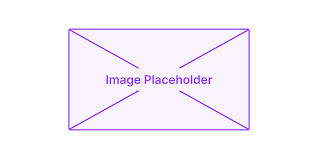
\includegraphics[width=15cm]{img/placeholder.png}
  \caption{ユニットのバリエーション}
  \label{fig:unit_valiation}
\end{figure}
\subsection*{マッピングの方法}
マッピングについては、1つの動きを複製して、1つの動きを複数のパーツの動きへと波及させるバリエーションなどを作成した。図\ref{fig:networked_finger}に示すプロトタイプでは、指先をクリックすると5本ある指のうちのいずれかの動きを追従する指が、指先に追加されるものである。どの指が付け加わるかはランダムで、指が新しく追加されるたびに、それがどの指の運動であるかを同定するには、一本一本指を動かして、どこがその指に対応しているのかについて同定する必要がある。
\begin{figure}[H]
  \centering
  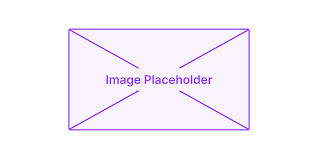
\includegraphics[width=15cm]{img/placeholder.png}
  \caption{Networked Finger}
  \label{fig:networked_finger}
\end{figure}

またそのほかに、図\ref{fig:fractal_finger}に示すプロトタイプでは、親指の先に人差し指の動きが複数分岐し、さらに人差し指の先から中指の動きが複数分岐して配置される、といったフラクタル構造で指の動きを配置したパターンを制作した。このように、配置を変えるだけでなく1つの指の動きに対して対応して動く部分を多数にするなどのバリエーションを検討した。

\begin{figure}[H]
  \centering
  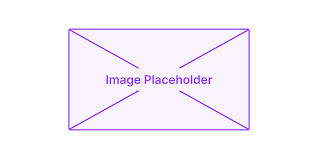
\includegraphics[width=15cm]{img/placeholder.png}
  \caption{Fractal Finger}
  \label{fig:fractal_finger}
\end{figure}
\subsection*{時間操作}
最新の自分の動きだけを表示するのではなく、過去の動きも表示するプロトタイプにも取り組んだ。図\ref{fig:prototype_delay}に示すプロトタイプでは、5本の指の動きが等間隔に並べられているが、それぞれの指は、鉛直上向きの角度に現在の指の動き、そこから時計回りに、順次過去の指の動きが並べられている\footnote{https://interaction005-moe5dbh11-k1105.vercel.app/}。

このプロトタイプでは、指先を小さく動かすと、その動きが時計回りに伝播していくようすが見て取れる。これは例えばゼリー状の物体を触れた時のような、衝撃が物体全体へと伝播していくようすに見立てられるため、柔らかいオブジェクトに触れているときのような身体感覚を錯覚することがある。

\subsection*{振り返り}

\begin{figure}[H]
  \centering
  
\includegraphics[width=15cm]{img/past_time.png}
  \caption{過去の動きを用いた例}
  \label{fig:prototype_delay}
\end{figure}
\subsection{表現の収束(執筆中)}
ここまで行なってきたプロトタイプから方向性を絞り、ブラッシュアップした。
\subsection*{動かしている感覚が強い表現}
1つ目の観点として、手指の微細かつ複雑な動きをもって、緻密な制御をしているという感覚が引き出される表現へと絞り込んでいくことにした。

その上で注目したのは、「関節を折り曲げる動き」に対する共感性である。
人間の手指は

その一方で、円の半径に関節の動きをマッピングさせるような表現については、縮んだり、膨らんだりする動きには共感しづらい。微細な運動が増幅される「気持ちよさ」があるが、この気持ちよさは身体動作との連動によってもたらされる気持ちよさではなく、動作に対するフィードバックに対する快、すなわちFelsのいう「Response」による快が強い。

また、1つの動きを複製して円形に配置したり、フラクタル的に配置するパターンを排除した。これについては、グラフィックデザイナーの女性が体験した際「構造としては緻密であるのに、動きは単純であるように感じる」と意見した。その理由として彼女は、「対称性が前面に出ているため、シンボルとしての印象を強く感じてしまう」「意識していないところも同時に動いている感覚があるため、自分の動きだと思えない」からではないかと推測した。

\subsection*{注意の対象による作品の分割}
一方で、プロトタイピングを通して同定した変換表現を通して生じた異なる身体像に対する共感覚のようなものは、変換された手を用いた作業に移行した瞬間に、注意が向きづらくなるといった課題が起こった。そこで、最終的な作品としてはその2つを分けて構成した。

\subsection*{モーフィング}
「身体の変容」を扱っている本作では、取得されたキーポイントの位置を大きく変更させることで、「意図的にIntimacyを下げる」操作を行なっている。しかし「下がった」という事実を体験者が認識するために、もとの手が鏡合わせのように出力されている状態から、徐々に形を変えていくようすを連続的に示すモーフィングを実装している。

過去に展示していたバージョンではモーフィングを示さず、手指が認識されたとたんに全く違う手指が提示される作品形態であった。しかし、この形態で展示した場合、画面の中の手指と自身の関係性について、全く異なる生命体のようなものを、操り人形のように自分の手指の指令によって動かす、といったような関係性として認識されることがあった。また、全く見慣れない形なので、「手指を細かく動かせる」といった、作品がもつ可能性に気づけない場合があることがわかった。そこで、このモーフィングを実装することで、白い点が関節を表していること、そして手指の運動を細かくトラッキングしていることを事前に伝え、それが形を変えた姿として画面の前に提示されていることを示す形態を採用することになった。
そうすることで、画面に出力されているグラフィックと身体との関係性は別々の存在ではなく、自分の身体であったことが明示される。

\subsection{展示形態の設計}
展示形態について、時系列順に過去2つのバージョンについて説明し、その流れから最終的な展示形態の根拠を示す。

\textbf{初期:カメラを画面前に配置した状態}\\
最初期は、体験装置について下図\ref{fig:kyotai_ver0}のように、モデルトラッキングを行っているカメラを直接画面の前に配置していた。
\begin{figure}[H]
  \centering
  \includegraphics[width=15cm]{img/kyotai_ver0.jpg}
  \caption{初期:カメラを画面前に配置した状態}
  \label{fig:kyotai_ver0}
\end{figure}

プロトタイピングの段階でもあったため最低限の構成としていたが、この構成には次のような問題があった。
\begin{quote}
  \begin{itemize}
    \item カメラのトラッキング精度が環境光の影響を受けて変動してしまう
    \item 体験者ではない周囲の人の手指を間違ってトラッキングしてしまう
    \item 手指の形がそのまま出力されるわけではないので、トラッキングの範囲がわからず、腕を大きく振ったり、手指がトラッキングできない範囲で動かしてしまう
  \end{itemize}
\end{quote}

このため、制作者が指示をすることなく自由に体験してもらうことを意図していた展示であっても、体験方法がわからなかったり、後方で見守る人の手を誤ってトラッキングしてしまうといった問題が起き、有効なフィードバックを得ることができなかった。

\textbf{中期:専用筐体を用いて手首を固定した状態}\\
こうした課題を踏まえて、次に専用筐体を制作し、穴に手を入れる形式について試した(図\ref{fig:kyotai_ver1})。

\begin{figure}[H]
  \centering
  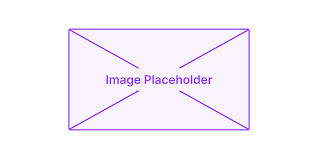
\includegraphics[width=15cm]{img/placeholder.png}
  \caption{中期:専用筐体を使用してカメラを隠蔽した状態}
  \label{fig:kyotai_ver1}
\end{figure}

この形式では、カメラの画角に映り込むのは筐体の内部と体験者の手のみであるため、環境光の影響や周囲の人の影響を受けずに体験してもらうことが可能となった。また、穴によって手首の位置が固定されるため、腕を大きく振ることが構造上不可能となり、比較的身体動作の幅が抑えられた。

ただし、この形式は単に上記の問題を解決したというだけではなく、指先の動きが見えなくなったこと、画面に対する指先の位置関係についてを変更するものであった。

画面に対する手指の位置関係については、本作品では手指の形状が、もとの形とは全く関係のない構造へと変化するため、作品体験には大きな影響はないと判断した。手指の動きが見えなくなったことについては、画面の中の手指は体験時、自身の身体に代わる存在であるから、同時に視認できない今の形態の方がむしろ、より適した構成であると判断した。

しかしその一方で、手首の動きを固定してしまったことは、身体の動きを過剰に限定してしまう結果となった。身体の動きを限定してしまうと、何か特定の動作を求められているような説明的な構成になってしまう。そのため筐体としては、より簡素な構成が好ましいと判断した。


\textbf{作品展示:専用筐体を用いて手首を固定せず指先を自由にした状態}\\
そこで最終的には、図\ref{fig:kyotai_ver2}のような、トラッキングの範囲を暗示しながら、手首を固定しない方式に変更した。また、トラッキングに用いるカメラを、視野角150°の広角カメラ(Sanwa Supply CMS-V43BK-3)に変更し、大きく手指を動かしてもトラッキングの外れることの少ないものへと変更した。

\begin{figure}[H]
  \centering
  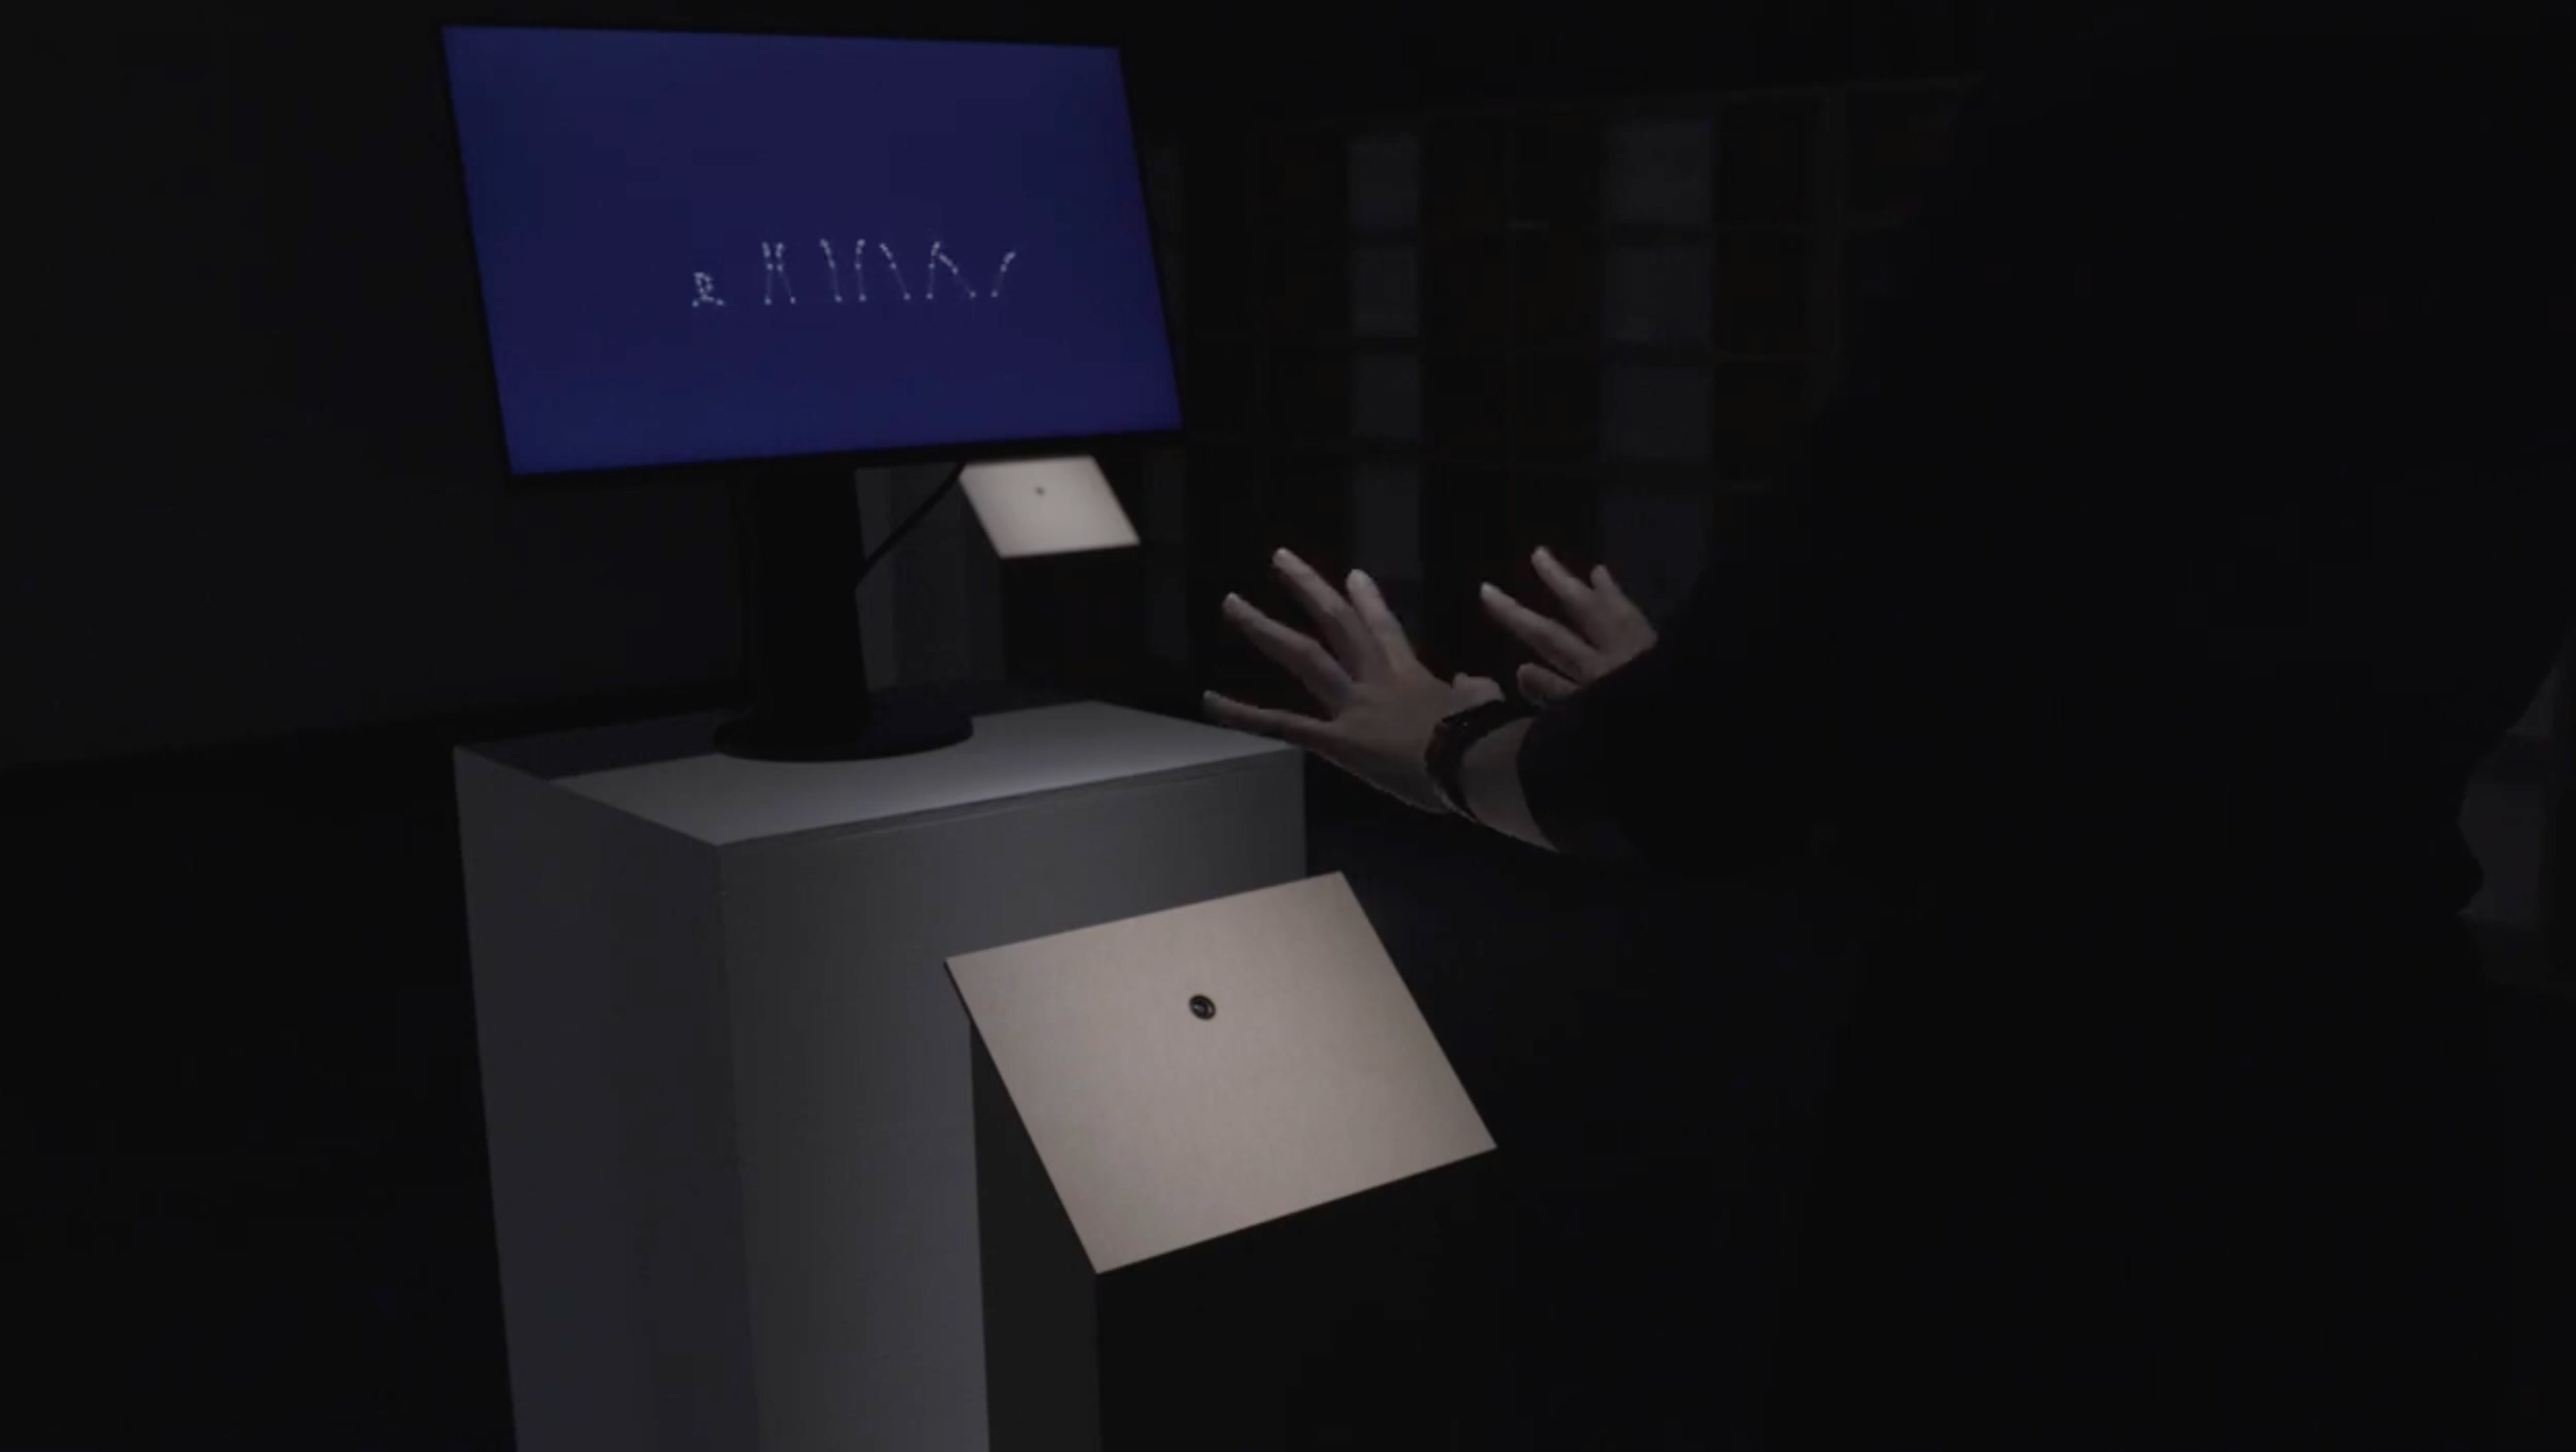
\includegraphics[width=15cm]{img/kyotai_ver2.png}
  \caption{作品展示の際の筐体}
  \label{fig:kyotai_ver2}
\end{figure}

筐体の高さは腰ほどの高さ(850mm)とすることで、キーボードのブラインドタッチのように、画面を見ながら手を同時に見ることが難しい構成とした。

カメラは、鉛直上向ではなく斜めを向いているので、筐体の前に立つと体験者の身体と手指の位置が重なり、トラッキングしやすい状況ができる。

また、ライティングの調整によってトラッキングの精度を高めた。
最終的な展示形態では、スポットライトを当てることで筐体周りを明るくすると同時に照り返しで手元の採光をし、周囲の照明を落とすことで明暗差を作ることで、手指の姿勢を認識しやすくなる。

\begin{figure}[H]
  \centering
  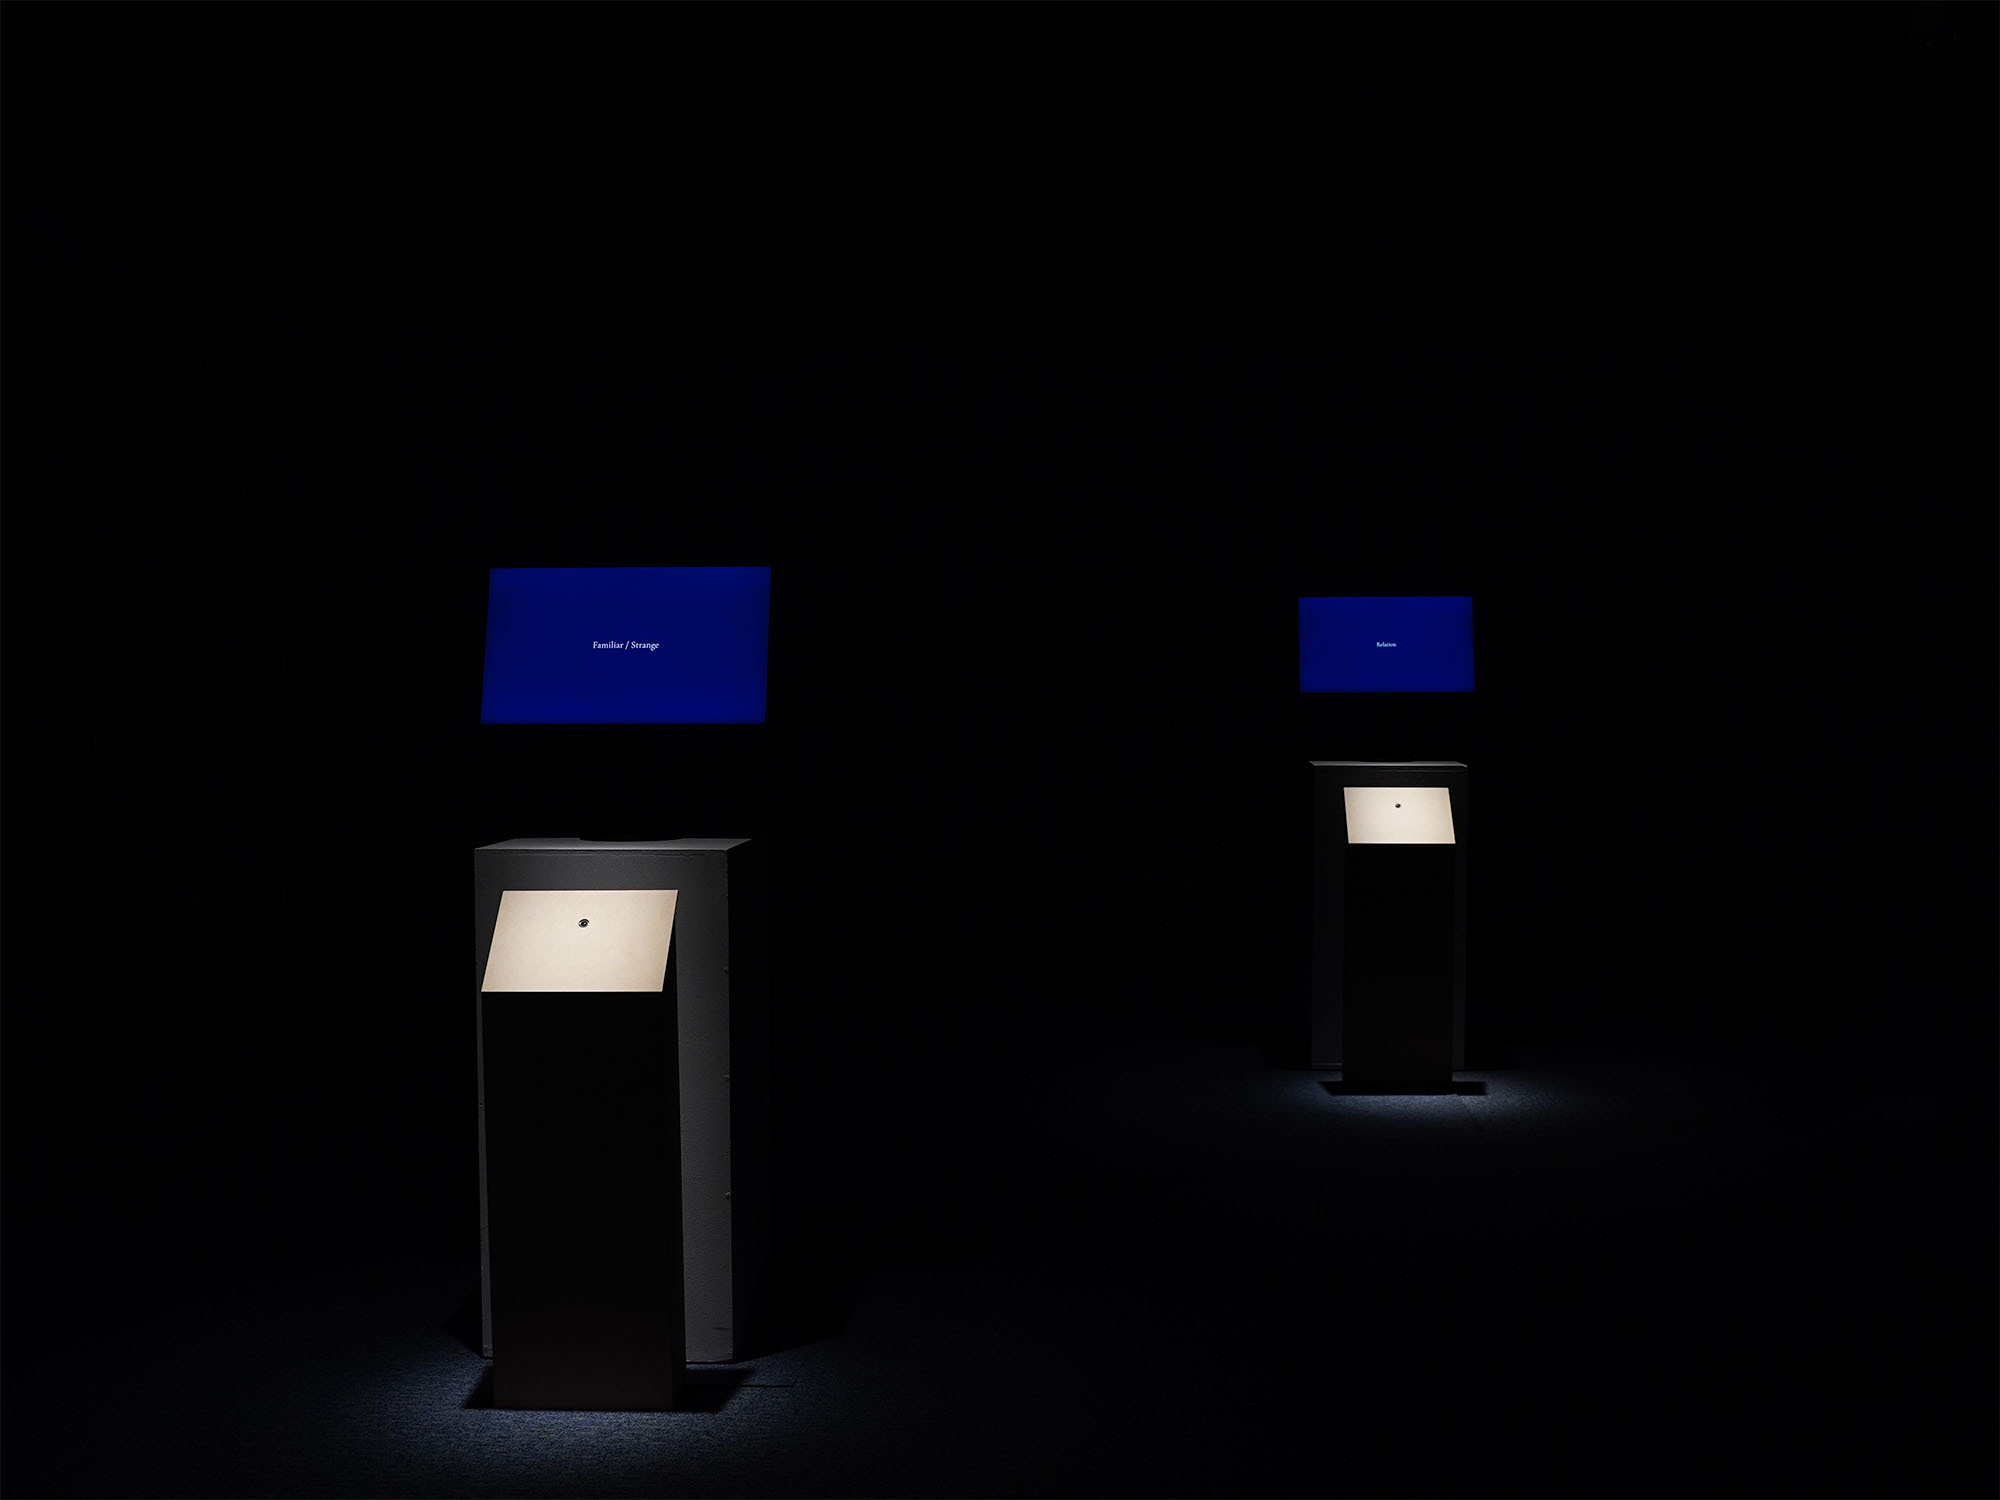
\includegraphics[width=15cm]{img/lighting.jpg}
  \caption{作品展示の際のライティング}
  \label{fig:lighting}
\end{figure}

\section{ライブラリの開発}
本作品を構成するにあたり、基本的な関数をまとめたライブラリを開発した。ライブラリには、円滑に体験するための補完処理を実装している。
具体的には、ガウシアンフィルターによる平滑化処理、トラッキングが途切れた際の例外処理の2つである。

\subsection{ガウシアンフィルターによる平滑化処理}
推定精度の問題から、モデルより推定される姿勢情報をそのまま出力すると、手指を動かしていなくても小刻みに振動したり、一時的なフレームレートの低下に起因してスムーズに動作していないように感じることがある。\\
そこで、体験者にフィードバックする際に使用する姿勢情報は、前後2フレーム分のフレーム情報にガウシアンフィルターを適用した平滑化処理を実装している。ただし、トラッキングが開始した直後は5フレーム分のフレーム情報を使用することができないため、この場合は取得できる限りのフレーム情報を用いて同じ処理を行なっている。そのため以下では、各フレーム情報に対する重みづけと、それを用いて体験者に提示される姿勢情報を求める上での一般式を示す。
モデルより推定された最新の姿勢情報を\(P_{n}\)、出力されている姿勢情報を\(S\)とすると、
  % 平滑化フレーム S の定義
  \begin{equation}
    S = \sum_{i=-2}^{2} w_i' \cdot P_{n+i}
    \end{equation}

ここで、\(w_i'\)は正規化されたガウシアンフィルタの重みを表す。正規化前の重み\(w_i\)は、
\begin{equation}
  w_i = \frac{1}{\sqrt{2\pi}\sigma} e^{-\frac{i^2}{2\sigma^2}}
  \end{equation}

正規化された重み\(w_i'\)は、
  % 重みの正規化
  \begin{equation}
  w_i' = \frac{w_i}{\sum_{j=-2}^{2} w_j}
  \end{equation}
と表現される。
この処理のため、最良時で60fps程度で取得される姿勢情報は、慢性的に0.3sほどの遅延を伴って体験者にフィードバックされることになる。

\subsection{トラッキングが途切れた際の例外処理}
体験時、環境光や、手指を動かす範囲や速度の関係から、トラッキングが途切れることがある。素早い動きをしている最中に1フレームでも途切れると円滑に体験することができないため、この時は例外的に、トラッキングが途切れる直前のフレーム情報で失われたフレーム情報を埋め合わせる処理を実装した。また、トラッキングが途切れていることに起因する不快感は、本作品の体験外の問題なので、手指の動きがトラッキングできていない状態を視覚的にフィードバックするため、トラッキング不能時に塗りつぶしを透過する視覚効果を実装した(\ref{fig:opacity})。

\begin{figure}[H]
  \centering
  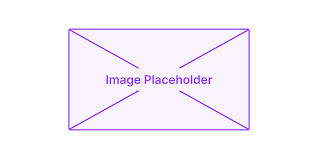
\includegraphics[width=15cm]{img/placeholder.png}
  \caption{トラッキング不能時の視覚効果}
  \label{fig:opacity}
\end{figure}
